\begin{minipage}[b]{0.6\textwidth}
\begin{Exercise}[label = rollingshutter, origin = Aaron Wild, difficulty = 3, title = Scannerlaufband]
	Ein Scanner kann man näherungsweise als eine sich von links nach rechts bewegte, senkrecht zur Bewegungsrichtung ausgedehnte Kamera betrachten, die eine kontinuierliche Aufnahme des Objekts auf dem Scannertisch macht.\\
	Die folgende Abbildung zeigt die Aufnahme einer Kreisscheibe, die entlang der Scannerachse bewegt wurde. Die Geschwindigkeit der Scannerkamera beträgt $v_s = 1~\mathrm{cm\cdot s^{-1}}$.
	Bestimme die Geschwindigkeit der Kreisscheibe $v_o$ und skizziere das Bild, was entsteht, wenn sie in die entgegengesetzte Richtung bewegt wird. Nimm dazu an, dass $v_o > v_s$ gilt.
\end{Exercise}
\end{minipage}
\begin{minipage}[b]{0.4\textwidth}
	\centering
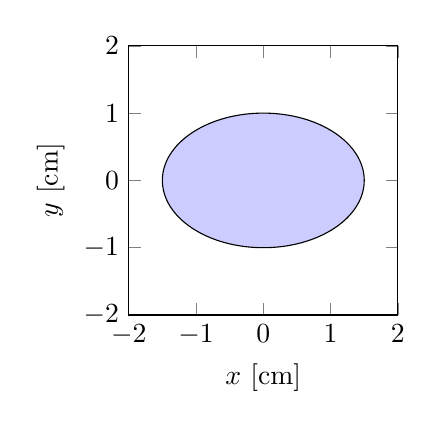
\begin{tikzpicture}
	\begin{axis}
	[xmin = -2,
	xmax = 2,
	ymin = -2,
	ymax = 2,
	width = 5cm,
	height = 5cm,
	xlabel = $x ~\lbrack \mathrm{cm}\rbrack$,
	ylabel = $y ~\lbrack \mathrm{cm}\rbrack$]
	\draw[fill = blue!20!white, draw = black] (axis cs: 0,0) circle [ x radius = 1.5,y radius = 1];
	\end{axis}
\end{tikzpicture}
\end{minipage}

\begin{Answer}[ref = rollingshutter]
	Durch die Scannerkamera findet keine Verzerrung des Bildes in $y$-Richtung statt, weil sie sich nur in $x$-Richtung bewegt. Dementsprechend kann man den Radius der Kreisscheibe sofort aus dem Bild zu $r = 1~\mathrm{cm}$ bestimmen. Der ursprüngliche Kreis wird somit durch die Gleichung 
	\begin{equation}\label{rollingshutter: circle}
		x^2 + y^2 = 1 ~\mathrm{cm}
	\end{equation}
	beschrieben.\\

	
\end{Answer}